\chapter{Advanced Techniques}

\section{Copy and Paste} \label{copy-paste}

Little Sound Dj has a clipboard for temporary data storage. Pressing \textsc{b+a} will cut the value
under the cursor and store it on the clipboard. The value can then be pasted by pressing
\textsc{select+a}.

In most screens, it is possible to mark up blocks by pressing \textsc{select+b} and moving around
the cursor. When having marked up a block, it can be copied to the clipboard by pressing \textsc{b},
or cut to the clipboard by pressing \textsc{select+a}. The clipboard contents can then be pasted by
pressing \textsc{select+a}.

Some quick-mark button presses are implemented:
\begin{itemize}
\item \textsc{select+(b, b)} = quick-mark a column or row.
\item \textsc{select+(b, b, b)} = quick-mark an entire screen.
\end{itemize}

When having marked a block, you can change all data inside that block by pressing \textsc{a+cursor}. This can be used, for example, to transpose several notes quickly.

\section{Cloning}

Cloning is a shortcut that can save you much unnecessary copy and paste action. It allows you to create copies of chains, phrases, instruments and tables directly from the song, chain, phrase and instrument screens.

Let's say you have a melody in chain 00, and you want to continue the song with the same melody, but a little changed. Then you copy 00 \textsc{(select+b, b)} and paste one row down \textsc{(select+a)}, so you get:

\begin{verbatim}
 00 
 00 
\end{verbatim}

Now, place the cursor on the second 00, and press \textsc{select+(b, a)}.
You will now get a new chain (probably called 01) which is a copy of 00. Since it's a copy, you can play around with it as much as you want without touching 00.

\subsection{Deep vs. Slim-Cloning}

There are two different modes for cloning: slim-cloning and deep-cloning. You can select the mode in the project screen.

If you slim-clone 00, Little Sound Dj makes a new chain 01 that
contains the same phrases as 00.

If you deep-clone 00, Little Sound Dj makes a new chain 00, and
also clones the phrases within 00 into 01. That way,
you can change 01's phrases without affecting 00.

The advantage of deep-cloning is that you have no risk of modifying old phrases by accident. The drawback is that it uses more phrases, so that you may run out of phrases faster. Also, your songs may take up more blocks when being saved using the file screen.

If you find yourself running out of phrases, try using \textsc{clean song data} in project screen. (Section \ref{clean-song-data}.)

\section{The Importance of Backups}

Some wise words from many peoples hard-earned experience: If you use Little Sound Dj on a Game Boy cartridge, it might be a good idea to examine backup options like the Transferer or the MegaMemory Card. Game Boy cartridges are often rather unstable, as they are depending on an internal battery that is likely to run out sooner or later. If you are serious about your music, you should do regular backups, or at least try to record your songs once in a while.

\section{Muting, Soloing and Panning on the Fly}

It is always possible to mute a channel temporarily by pressing \textsc{b+select}. If the \textsc{b} button is released before \textsc{select}, the channel will stay muted until \textsc{b} is pressed again. 

Correspondingly, a channel can be played solo by pressing \textsc{b+start}. If the \textsc{b} button is released before \textsc{start}, the other channels will stay muted. If the \textsc{start} button is released first, all channels will be turned on again.
 
It is also possible to pan channels left or right, by pressing \textsc{b+left/right} in the song screen.

\section{Live Mode}

 The live mode is a special flavor of the song screen. It can be reached by pressing \textsc{select+left} while in the song screen. In the live mode, it is possible to start and stop playing chains one by one. In contrast to the usual song screen, the different channels can be started and stopped independently. It is also possible to jump between different song positions while playing, without causing audio glitches or lost synchronization.

To play a chain, move the cursor to the chain and press \textsc{start}. To stop playing a chain, go to that channel and press \textsc{select+start}. If another chain is already playing, the starts and stops will be queued until that chain has been played through. If you want to queue until the next phrase end instead, tap \textsc{start} twice to speed up the switch.

To switch back to song mode from live mode, just press \textsc{select+left} while in the song screen.


\includegraphics[width=1cm]{tip}TIP!
\begin{itemize}
        \item \textit{To start or stop several chains at once, mark them before pressing \textsc{start} or \textsc{select+start}. (Marking is described in section \ref{copy-paste}.)}
	\end{itemize}

\subsection{Chain Loops}

 Using chain loops is a useful live mode technique. This technique is based on the fact that the song sequencer (when being in the live mode) won't rewind the song position all the way up to the first song sequencer step when encountering end of track; instead, it stops rewinding as soon as it encounters an empty step.

\begin{figure}[htpb]
	\begin{center}
	\fbox{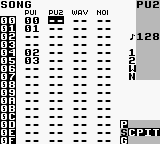
\includegraphics{chainloop}}
	\end{center}
	\caption{Chain Loop Example}
	\label{fig:chainloop}
\end{figure}

Example: We have a setup that looks like figure~\ref{fig:chainloop}.

Assume that we start playing pulse channel 1 at song position 4. The player will now loop chains 2 and 3. Defining a number of such chain loops to alternate between would provide a good starting point for a live performance.

\section{Creating Synthetic Drum Instruments}

Creating good-sounding drum instruments without using the sampled drum kits might be a bit tricky, if you've had no prior experience with drum synthesis. Nevertheless, it's a very useful technique once you know it. Here are some starting-out ideas.

\begin{figure}[hbtp]
	\centering
	\subfloat[Bass Drum]{
		\fbox{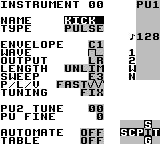
\includegraphics{instr-kick}}
	}
	\qquad
	\subfloat[Snare Drum]{
	\fbox{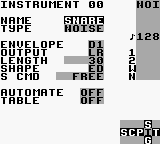
\includegraphics{instr-snare}}
	}

	\subfloat[Closed Hi-Hat]{
		\fbox{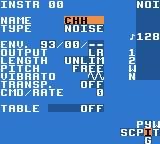
\includegraphics{instr-chh}}
	}
	\qquad
	\subfloat[Open Hi-Hat]{
	\fbox{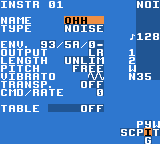
\includegraphics{instr-ohh}}
	}

	\subfloat[Cymbal]{
		\fbox{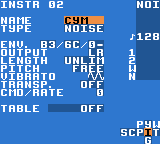
\includegraphics{instr-cym}}
	}
	\qquad
	\subfloat[Snare Drum Table]{
	\fbox{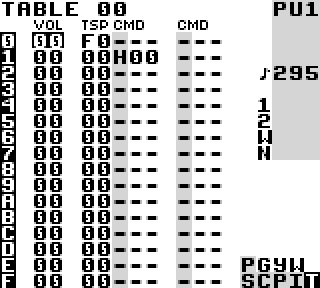
\includegraphics{table-snare}} \label{fig:table-snare}
	} 

	\caption{Synthetic Drum Instruments}
	\label{fig:instr-examples}
\end{figure} 

\subsection{Bass Drum}

Use pulse channel 1 for creating bass drum sounds. The amplitude envelope should have a strong attack and fast decay - try setting it to \$C1. Wave should be 50-50 high/low, even though other waves can be used for making the instrument sound more distorted. The sweep value is maybe the most important part in creating a successful kick instrument. It should have a high initial frequency and decay. Try setting it to a value of \$E3, and playing the instrument at note C-6. For a more snappy sounding kick, try experimenting with the envelope and length parameters.

It is also possible to use the noise channel for creating bass drums. Feel free to experiment around.

\subsection{Snare Drum}

Use the noise channel for creating snare drum sounds. The amplitude envelope should have a strong attack and fast decay - try setting it to \$C1. Use the length parameter to create more snappy sounding snares. The shape parameter can be used for adjusting the timbre - shape values close to \$EC might prove useful. 

\subsection{Hi-Hats and Cymbals}

Hi-hats are created using the noise channel. Use a shape value of \$FF for selecting a timbre with high frequency content. Change the envelope and length parameters for creating the desired amplitude envelope. For emulating cymbals, use a shape value near \$EE to create a somewhat rougher timbre.

\subsection{Taking Advantage of Tables}

For adding that extra punch to snares, you can use a table that uses the transpose column to change the noise shape rapidly. (See figure~\ref{fig:table-snare}.) 



